\documentclass[a4paper, 12pt, leqno]{report}

\usepackage[T1]{fontenc}
\usepackage[utf8x]{inputenc}
\usepackage[greek,french]{babel}
\usepackage[babel=true]{csquotes}
\usepackage[top=1.5cm, bottom=2.0cm, left=2.0cm, right=2.0cm]{geometry}
\usepackage{fancyhdr}
\usepackage{graphicx}
\usepackage{amsmath}
\usepackage{soul}
\usepackage{amssymb}
\pagestyle{plain}
\usepackage{amsfonts}
\usepackage{amssymb}
\usepackage{amsthm}
\usepackage{graphicx}
\usepackage{color}
\usepackage{enumerate}
\usepackage{array}
\theoremstyle{plain}
\usepackage{blkarray}
\usepackage{listings}
\usepackage{algorithmicx}
\usepackage{algpseudocode}
\usepackage{algorithm}

\usepackage{caption}
\DeclareCaptionFont{white}{\color{white}}
\DeclareCaptionFormat{listing}{\colorbox{black}{\parbox{\textwidth}{#1#2#3}}}
\captionsetup[lstlisting]{format=listing,labelfont=white,textfont=white}


\newcommand{\bigO}[1]{\ensuremath{\mathop{}\mathopen{}O\mathopen{}\left(#1\right)}}
\newcommand{\smallO}[1]{\ensuremath{\mathop{}\mathopen{}o\mathopen{}\left(#1\right)}}

\title{\textsc{\textbf{Rapport TP n°2 IA01}}}
\author{\textbf{Damien MARI\'E et Antoine POUILLAUDE}}

\begin{document}
    \maketitle
    \tableofcontents
\newpage
\section*{Remarques générales}
		Ce TP, bien que pas facile, nous a ammener à implémenter des fonctions de parcours d'états en fonction de conditions fixées au départ. C'est-à-dire que nous devions à chaque fois que l'on changeait d'état vérifier si l'état était cohérent par rapport à l'ennoncé qui nous été donné. C'est, au final, un TP très instructif et amusant même.
        \chapter{Préparation du problème}  
        \section{Question n°1}      
            Suivons le formalisme donné dans l'ennoncé. Un état est ainsi représenté : (État rive gauche, État rive droite) sachant qu'un état d'une rive est donné par (nombre de Missionnaire, nombre de Cannibale, 1 si le bâteau est amarré à la rive 0 sinon). Ainsi nous obtenons l'ensemble des états : 
            \[ \text{Ensemble d'état} = 
            \{ ((3\ 3\ 1) (0\ 0\ 0)),
            ((2\ 2\ 0) (1\ 1\ 1)),
            ((3\ 2\ 1) (0\ 1\ 0)),
            ((0\ 1\ 0) (3\ 2\ 1)),
            ...
            \}\]
            
    Cela dit on remarque très vite que la notation est lourde et futile puisque dans tous les cas on doit avoir : 
\[
          \left\{
    \begin{array}{ll}
        \sum_{\{Rive gauche,Rive droite\}}^{}Cannibale =3\\
        et\\
        \sum_{\{Rive gauche,Rive droite\}}^{}Missionaire = 3
    \end{array}
\right.
\forall \text{ etat } \in \text{Ensemble d'état}
\]
Alors on pourrait simplifier la liste des états. Du moment que l'on connait l'état d'une on peut alors connaitre l'état de l'autre rive par déduction. Par conséquent, nous simplifierons en affichant l'état que d'un seul côté. Ainsi on aura l'ensemble des états suivant :
\[ \text{Ensemble d'état} = 
            \{ (3\ 3\ 1),
            (2\ 2\ 0),
            (3\ 2\ 1),
            (3\ 2\ 0),
            (0\ 1\ 0),
            (2\ 3\ 1),
            (2\ 3\ 0),
            (1\ 1\ 1),
            ...
            \}\]

		\section{Question n°2}     
            On donne l'ensemble des opérateurs comme suit :
               $$
               \left\{
    \begin{array}{ll}
    *R-ops* <= ((0\ 1)\ (1\ 0)\ (1\ 1)\ (2\ 0)\ (0 2))\\     
                *L-ops* <= ((0\ -1)\ (-1\ 0)\ (-1\ -1)\ (-2\ 0)\ (0\ -2))
    \end{array}
    \right.
    $$
    Bien sûr on a fait la distinction entre les opérations que l'ont peut effectué sur la rive gauche et droite. Les opérations dangereuses pour les missionaires sont, d'une manière générale celles durant lesquels des missionnaires sont déplacés d'un bord à l'autre sans pour autant que des cannibales soient déplacés. 
        
        \newpage
        \section{Question n°3} 
        On donne l'état initial comme ceci :
            \[(3\ 3\ 1)\]
            On a également l'état final :
            \[(0\ 0\ 0)\]
            
            \section{Question n°4}
            
            \begin{figure}[h]
            \begin{center}
            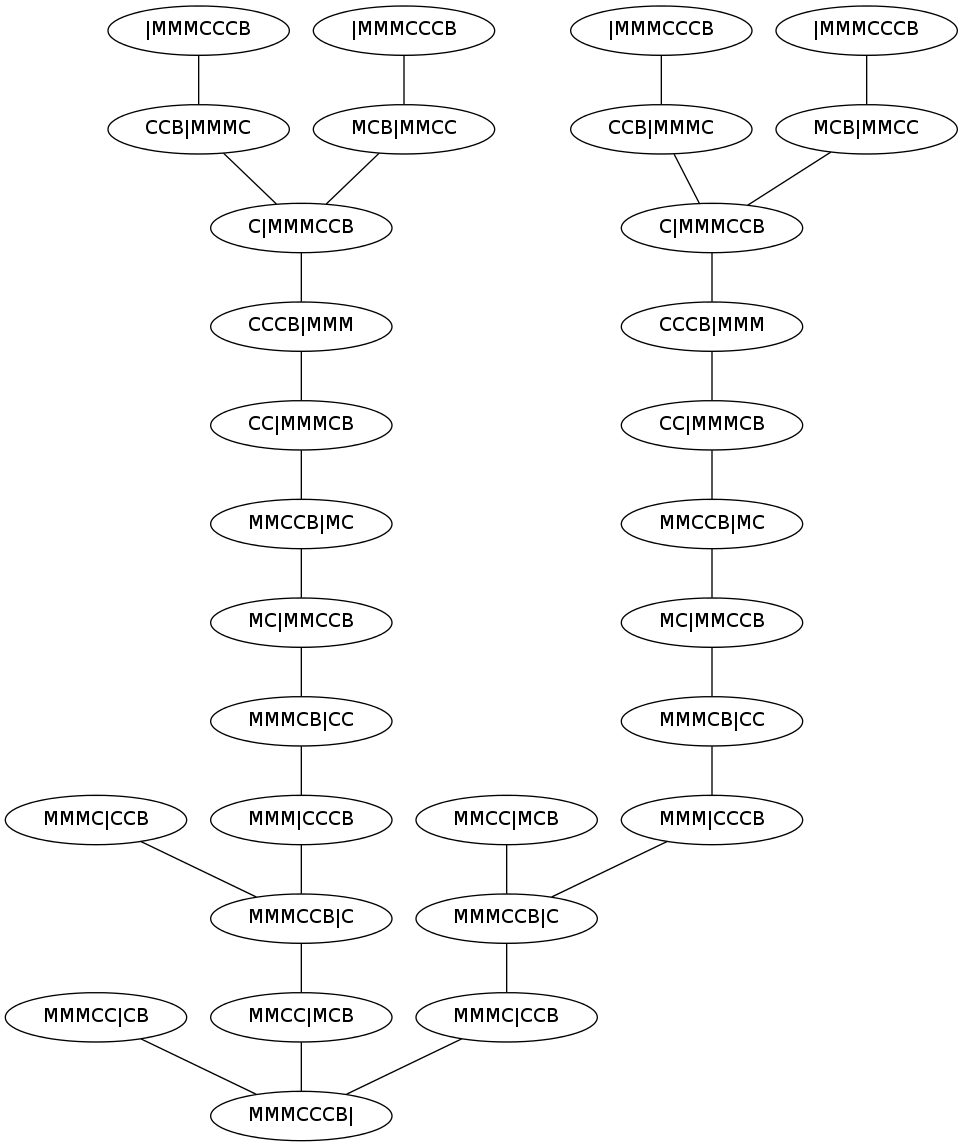
\includegraphics[scale=0.40]{graph.png}
            \end{center}
            \caption{Arbre de résolution partiel}
            \label{Arbre de résolution partiel}
            \end{figure}
            
            
             \chapter{Parcours de l'arbre pour trouver les solutions}
             On donne à présent les algorithmes pour la résolution de ce problème. Nous avons tenté de programmer l'algorithme des deux façons qui nous étaient proposés : parcours en largeur d'abord et en profondeur d'abord.
             
             Mais définissons tout d'abord les fonctions de services et les variables associés aux problèmes.
             
             \section{Les opérations}
             On donne la déclaration en lisp des listes correspondantes aux opérations que l'ont peut effectuer sur les états en fonction de la rive sur laquelle se trouve le bâteau.
             \begin{lstlisting}[label=some-code,caption=Déclaration des opérations ,language=lisp]
(setq *R-ops* '((0 1) (1 0) (1 1) (2 0) (0 2))) 
(setq *L-ops* '((0 -1) (-1 0) (-1 -1) (-2 0) (0 -2)))
            \end{lstlisting} 
            \section{Vérifier les états}
            Voici la fonction qui vérifie si un états est correct ou non.  
             \begin{lstlisting}[label=some-code,caption=verify (state) ,language=lisp]
(defun verify (state)
  (cond
    ((or (< (car state) 0) (< (cadr state) 0)) nil)
    ((or (> (car state) 3) (> (cadr state) 3)) nil)
    (
      (and 
        (and (not (= (car state) 3)) (not (= (car state) 0)))
        (not (= (car state) (cadr state)))
      )
      nil
    )
    (T T)
  )	
)
            \end{lstlisting} 
            \newpage
            Ces conditions ont été déduites du tableau suivant 
            \begin{center}
            \begin{tabular}{|c|c|c|}
            \hline
            Nombre de Missionnaire & Nombre de Cannibale & État\\ \hline
            0&0&OK\\ \hline 1&0&Incorrect\\ \hline 2&0&Incorrect\\ \hline 3&0&OK\\ \hline
            0&1&OK\\ \hline 1&1&OK\\ \hline 2&1&Incorrect\\ \hline 3&1&OK\\ \hline
            0&2&OK\\ \hline 1&2&Incorrect\\ \hline 2&2&OK\\ \hline 3&2&OK\\ \hline
            0&3&OK\\ \hline 1&3&Incorrect\\ \hline 2&3&Incorrect\\ \hline 3&3&OK\\
            \hline
            \end{tabular}
               \end{center}
               
            \section{La fonction d'inclusion}
            Cette fonction permet de savoir si un état appartient à l'ensemble des états déjà visités.
             \begin{lstlisting}[label=some-code,caption=in (x L) version récursive ,language=lisp]
(defun in (x L)
  (if (or (eq x nil) (eq L nil)) NIL (if (equal (car L) x) T (in x (cdr L))))
)
            \end{lstlisting} 
            \section{Applications des opérations à l'état courant}
            Cette fonction va permettre d'avoir le résultat de l'application des opérations choisies sur l'état courant.
            \begin{lstlisting}[label=some-code,caption=apply-op (state op) ,language=lisp]
(defun apply-op (state op)
  (list 
    (+ (car state) (car op)) 
    (+ (cadr state) (cadr op)) 
    (if (eq (caddr state) 1) 0 1))
)
            \end{lstlisting}
            
            \newpage
            
            \section{Parcours en largeur d'abord} 
            \subsection{Fonctions pour enfiler et défiler}
            Les deux fonctions suivantes vont servirent à enfiler et à défiler des éléments dans une file FIFO afin de pouvoir par la suite implémenter la fonction de parcours en largeur d'abord. Cependant, on aurait, après réflexion, utiliser utiliser les fonctions de bases de lisp pour arriver à nos fins.
            \subsubsection{Enfiler}
            \begin{lstlisting}[label=some-code,caption=enqueue (x Q) ,language=lisp]
(defun enqueue (x Q)
  (if (null Q)
    (list x)
	(nconc Q (list x))
  )
)
            \end{lstlisting}
            \subsubsection{Défiler}
            \begin{lstlisting}[label=some-code,caption=dequeue (Q) ,language=lisp]
(defun dequeue (Q)
  (cdr Q)
)
            \end{lstlisting}
            
            \subsection{Fonction de parcours}
            Voici donc la tant attendue fonction de parcours qui au terme de son execution doit donner les manières de résoudre le problème donné.
            \subsubsection{Algorithme}
            \begin{algorithm}
            \caption{Algorithme de parcours en largeur d'abord}
            \begin{algorithmic}
            \While{Q is not empty}
            \State node := Q[1]
            \State dequeue(Q)
            \If {$car(x) = (0\ 0\ 0)$}
                \State retourner $cadr(node) + (0\ 0\ 0)$
            \ElsIf {$verify(car\ node)$}
                     \ForAll{$x \in \left\{\begin{array}{ll}*R-ops*&\text{si }cadr(car(node))=0\\
                     *L-ops*&\text{si }cadr(car(node))=1 \end{array}\right.
$}
            \State res := $apply-op(car(node),op)$
            \If {$not\ in(res,cadr(node))$ and $verify(res)$}
                    \State Q := $\left\{\begin{array}{ll}
                    enqueue(((res)\ (car(node))),Q)&\text{si }cadr(node)=NIL\\
                    enqueue(((res)\ (cadr(node) +car(node))),Q)&\text{sinon}
                    \end{array}\right.$
            \EndIf
            \EndFor
            \EndIf   
            \EndWhile
            \end{algorithmic}
            \end{algorithm}  
            \subsubsection{Implémentation en lisp}
            \begin{lstlisting}[label=some-code,caption=BFS-solve (N L) version largeur d'abord,language=lisp]
(defun BFS-solve (Q)
  (dolist (node Q)
    (setq Q (dequeue Q))
      (cond 
	    ((equal (car node) '(0 0 0)) 
	      (print "Solution: ") 
	      (print (append (cadr node) (list '(0 0 0)))))  
	    ((verify (car node)) 
	      (dolist 
	        (op (if (eq (caddr (car node)) 0) *R-ops* *L-ops*))
	        (setq res (apply-op (car node) op))
	        (if (and (not (in res (cadr node))) (verify res))
              (if (eq (cadr node) NIL)	
	            (setq Q (enqueue (list res (list (car node))) Q))
	            (setq Q 
	              (enqueue (list res 
	              (append (cadr node) 
	              (list (car node)))) 
	              Q
	            )
	          )
	        )
	      )	
	    )
	  )
	)
  )
)
(if (null Q) "END" (BFS-solve Q))	
)
            \end{lstlisting}
          Après l'execution de cette fonction nous obtenons bien les 4 solutions que nous attendions selon l'arbre dessiné plus haut.
            \begin{lstlisting}[label=some-code,caption=Résultat d'execution de la fonction de parcours en largeur d'abord.,language=lisp]
"Parcours en largeur" 
"Solution:" 
((3 3 1) (2 2 0) (3 2 1) (3 0 0) (3 1 1) (1 1 0) (2 2 1) (0 2 0) (0 3 1)
 (0 1 0) (0 2 1) (0 0 0)) 
"Solution:" 
((3 3 1) (2 2 0) (3 2 1) (3 0 0) (3 1 1) (1 1 0) (2 2 1) (0 2 0) (0 3 1)
 (0 1 0) (1 1 1) (0 0 0)) 
"Solution:" 
((3 3 1) (3 1 0) (3 2 1) (3 0 0) (3 1 1) (1 1 0) (2 2 1) (0 2 0) (0 3 1)
 (0 1 0) (0 2 1) (0 0 0)) 
"Solution:" 
((3 3 1) (3 1 0) (3 2 1) (3 0 0) (3 1 1) (1 1 0) (2 2 1) (0 2 0) (0 3 1)
 (0 1 0) (1 1 1) (0 0 0))  
            \end{lstlisting}             
        \section{Parcours en profondeur d'abord}
                    La fonction suivante sert à parcourir les états mais cette fois-ci en profondeur d'abord. En revanche, la fonction ne renvoi le résultat attendu et nous ne savons pas pourquoi.
             \subsubsection{Algorithmique}     
             \begin{algorithm}
            \caption{Algorithme de parcours en profondeur d'abord}
            \begin{algorithmic}
            \If {$car(x) = (0\ 0\ 0)$}
                \State retourner $previous-states + (0\ 0\ 0)$
            \ElsIf {$not\ verify(state)$}
                \State retourner NIL
            \Else   
                \ForAll{$x \in \left\{\begin{array}{ll}*R-ops*&\text{si }cadr(car(node))=0\\
                     *L-ops*&\text{si }cadr(car(node))=1 \end{array}\right.
$}
            \State res := $apply-op(car(node),op)$
            \If {$not\ in(res,cadr(node))$ and $verify(res)$}
                    \State retourner $\left\{\begin{array}{ll}
                    DFS-solve(res,(state))&\text{si }previous-states=NIL\\
                    DFS-solve(res,previous-states+state)&\text{sinon}
                    \end{array}\right.$
            \EndIf
            \EndFor
            \EndIf   
            \end{algorithmic}
            \end{algorithm}  
            \subsubsection{Implémentation en lisp}        
            \begin{lstlisting}[label=some-code,caption=DFS-solve (state previous-states) version profondeur d'abord,language=lisp]
(defun DFS-solve (state previous\-{}states)
  (cond
    ((equal state '(0 0 0))
      (print "Solution:")
      (print (nconc previous\-{}states (list '(0 0 0)))))
     ((not (verify state)) nil)
     (T
       (dolist 
         (op (if (eq (caddr state) 0) *R-ops* *L-ops*))
         (setq res (apply\-{}op state op))
         (if (and (not (in res previous\-{}states)) (verify res))
           (if (null previous-states)
             (DFS-solve res (list state))
             (DFS-solve res (nconc previous-states (list state)))
           )
         )
       )
     )
   )  
)
            \end{lstlisting}
          $previous-states$ reprèsente les états déjà visités durant le parcours et $state$ reprèsente l'état courant.\newpage
          Après l'excution de la fonction on obtiens le résultat suivant.
            \begin{lstlisting}[label=some-code,caption=Résultat d'execution de la fonction de parcours en profondeur d'abord.,language=lisp]
"Solution:" 
((3 3 1) (2 2 0) (3 2 1) (3 2 1) (3 0 0) (3 1 1) (1 1 0) (2 2 1) (0 2 0)
 (0 3 1) (0 1 0) (0 2 1) (0 0 0)) 
"Solution:" 
((3 3 1) (3 1 0) (3 2 1) (3 2 1) (3 0 0) (3 1 1) (1 1 0) (2 2 1) (0 2 0)
 (0 3 1) (0 1 0) (0 2 1) (0 0 0)) 
            \end{lstlisting}       

                
\end{document}
